\chapter{Execution of a PASS Model}
\label{PASSExec}

\section{Informal Description of Subject Behavior and its Execution}
The excution of subject means sending and reveiving messages and executing internal activities in the defined order. In the following sections it is described what sending and receiving messages and executing internal functions means.

\subsection{Sending Messages}
Before sending a message, the values of the parameters to be transmitted need to be determined. In case the message parameters are simple data types, the required values are taken from local variables or business objects of the sending subject, respectively. In case of business objects, a current instance of a business object is transferred as a message parameter.\\
The sending subject attempts to send the message to the target subject and store it in its input pool. Depending on the described configuration and status of the input pool, the message is either immediately stored or the sending subject is blocked until a delivery of the message is possible.\\
In the sample business trip application, employees send completed requests using the message ‘send business trip request’ to the manager’s input pool. From a send state, several messages can be sent as an alternative. The following example shows a send state in which the message M1 is sent to the subject S1, or alternatively the message M2 is sent to S2, therefore referred to as alternative sending (see Figure \ref{fig:sendstate}). It does not matter which message is attempted to be sent first. If the send mechanism is successful, the corresponding state transition is executed. In case the message cannot be stored in the input pool of the target subject, sending is interrupted automatically, and another designated message is attempted to be sent. A sending subject will thus only be blocked if it cannot send any of the provided messages.

\begin{figure}[ph]
	\centering
	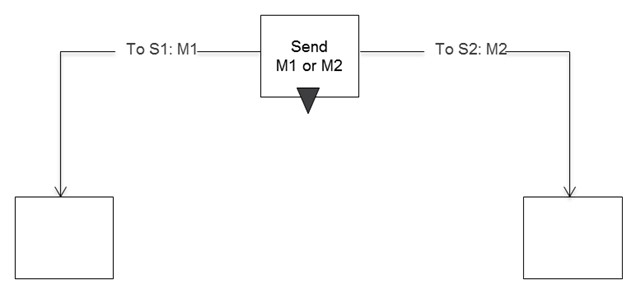
\includegraphics[width=0.7\linewidth]{20181026-Ontologie-Bilder/Grafiken-Ontologie/SUbjectExecution/sendState}
	\caption[Example of alternative sending]{Example of alternative sending}
	\label{fig:sendstate}
\end{figure}

By specifying priorities, the order of sending can be influenced. For example, it can be determined that the message M1 to S1 has a higher priority than the message M2 to S2. Using this specification, the sending subject starts with sending message M1 to S1 and then tries only in case of failure to send message M2 to S2. In case message M2 can also not be sent to the subject S2, the attempts to send start from the beginning.

The blocking of subjects when attempting to send can be monitored over time with the so-called timeout. The example in Figure \ref{fig:sendstatetimer} shows with ‘Timeout: 24 h’ an additional state transition which occurs when within 24 hours one of the two messages cannot be sent. If a value of zero is specified for the timeout, the process immediately follows the timeout path when the alternative message delivery fails completely.

\begin{figure*}[ph]
	\centering
	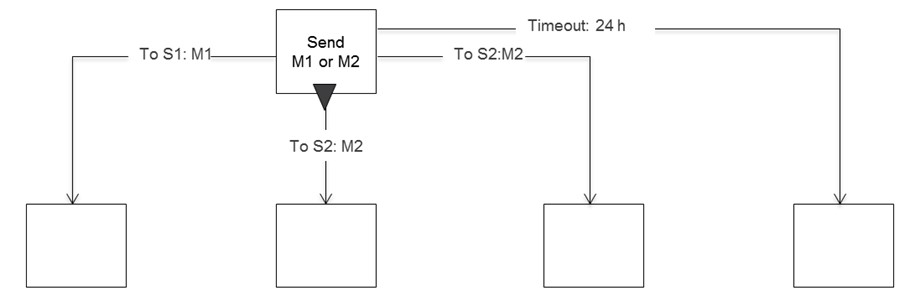
\includegraphics[width=0.7\linewidth]{20181026-Ontologie-Bilder/Grafiken-Ontologie/SUbjectExecution/SendSTateTimer}
	\caption[Send using time monitoring]{Send using time monitoring}
	\label{fig:sendstatetimer}
\end{figure*}


\subsection{Receiving Messages}
Analogously to sending, the receiving procedure is divided into two phases, which run inversely to send.

The first step is to verify whether the expected message is ready for being picked up. In case of synchronous messaging, it is checked whether the sending subject offers the message. In the asynchronous version, it is checked whether the message has already been stored in the input pool. If the expected message is accessible in either form, it is accepted, and in a second step, the corresponding state transition is performed. This leads to a takeover of the message parameters of the accepted message to local variables or business objects of the receiving subject. In case the expected message is not ready, the receiving subject is blocked until the message arrives and can be accepted.

In a certain state, a subject can expect alternatively multiple messages. In this case, it is checked whether any of these messages is available and can be accepted. The test sequence is arbitrary, unless message priorities are defined. In this case, an available message with the highest priority is accepted. However, all other messages remain available (e.g., in the input pool) and can be accepted in other receive states.

Figure \ref{fig:receivestate} shows a receive state of the subject ‘employee’ which is waiting for the answer regarding a business trip request. The answer may be an approval or a rejection.

\begin{figure*}[ph]
	\centering
	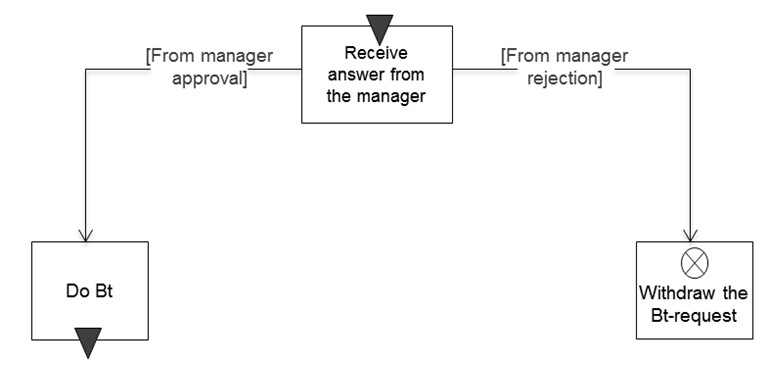
\includegraphics[width=0.7\linewidth]{20181026-Ontologie-Bilder/Grafiken-Ontologie/SUbjectExecution/ReceiveState}
	\caption[Example of alternative receiving]{Example of alternative receiving}
	\label{fig:receivestate}
\end{figure*}

Just as with sending messages, also receiving messages can be monitored over time. If none of the expected messages are available and the receiving subject is therefore blocked, a time limit can be specified for blocking. After the specified time has elapsed, the subject will execute the transition as it is defined for the timeout period. The duration of the time limit may also be dynamic, in the sense that at the end of a process instance the process stakeholders assigned to the subject decide that the appropriate transition should be performed. We then speak of a manual timeout.

\begin{figure*}[ph]
	\centering
	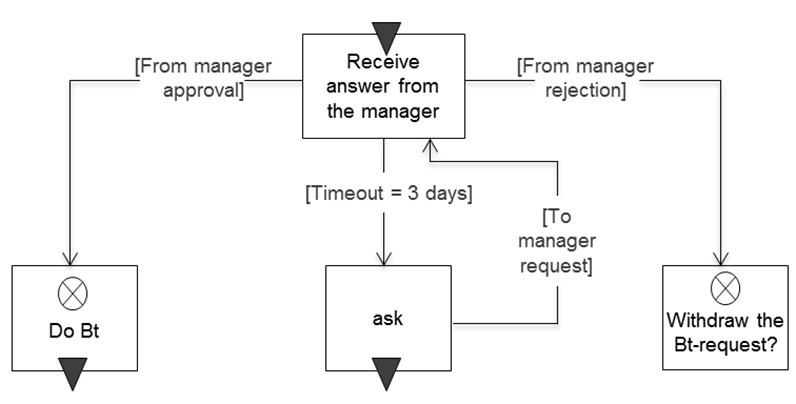
\includegraphics[width=0.7\linewidth]{20181026-Ontologie-Bilder/Grafiken-Ontologie/SUbjectExecution/ReceiveStateTimer}
	\caption[Time monitoring for message reception]{Time monitoring for message reception}
	\label{fig:receivestatetimer}
\end{figure*}

\newpage
Figure \ref{fig:receivestatetimer} shows that, after waiting three days for the manager’s answer, the employee sends a corresponding request.

Instead of waiting for a message for a certain predetermined period of time, the waiting can be interrupted by a subject at all times. In this case, a reason for abortion can be appended to the keyword ‘breakup’. In the example shown in Figure \ref{fig:receivestatebreak}, the receive state is left due to the impatience of the subject.

\begin{figure*}[ph]
	\centering
	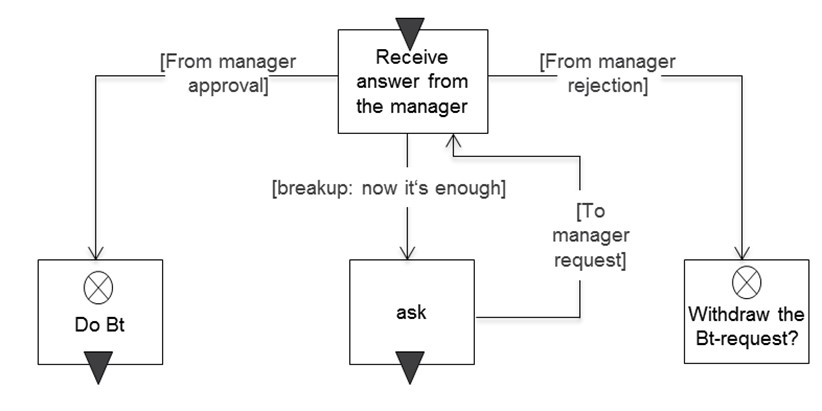
\includegraphics[width=0.7\linewidth]{20181026-Ontologie-Bilder/Grafiken-Ontologie/SUbjectExecution/ReceiveStateBreak}
	\caption[Message reception with manual interrupt]{Message reception with manual interrupt}
	\label{fig:receivestatebreak}
\end{figure*}
\newpage

\subsection{Standard Subject Behavior}
The possible sequences of a subject’s actions in a process are termed subject behavior. States and state transitions describe what actions a subject performs and how they are interdependent. In addition to the communication for sending and receiving, a subject also performs so-called internal actions or functions.

States of a subject are therefore distinct: There are actions on the one hand, and communication states to interact with other subjects (receive and send) on the other. This results in three different types of states of a subject. Figure \ref{fig:behavior-symbole} shows the different types of states with the coresponding symbols.

\begin{figure*}[ph]
	\centering
	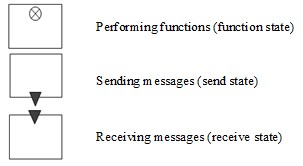
\includegraphics[width=0.5\linewidth]{20181026-Ontologie-Bilder/Grafiken-Ontologie/SUbjectExecution/Behavior-Symbole}
	\caption[State types and coresponding symbols]{State types and coresponding symbols}
	\label{fig:behavior-symbole}
\end{figure*}

In S-BPM, work performers are equipped with elementary tasks to model their work procedures: sending and receiving messages and immediate accomplishment of a task (function state).
In case an action associated with a state (send, receive, do) is possible, it will be executed, and a state transition to the next state occurs. The transition is characterized through the result of the action of the state under consideration: For a send state, it is determined by the state transition to which subject what information is sent. For a receive state, it becomes evident in this way from what subject it receives which information. For a function state, the state transition describes the result of the action, e.g., that the change of a business object was successful or could not be executed.

The behavior of subjects is represented by modelers using Subject Behavior Diagrams (SBD). Figure \ref{fig:vollst-beispiel} shows the subject behavior diagram depicting the behavior of the subjects ‘employee’, ‘manager’, and ‘travel office’, including the associated states and state transitions. 

\begin{landscape}
\begin{figure}[ph]
	\centering
	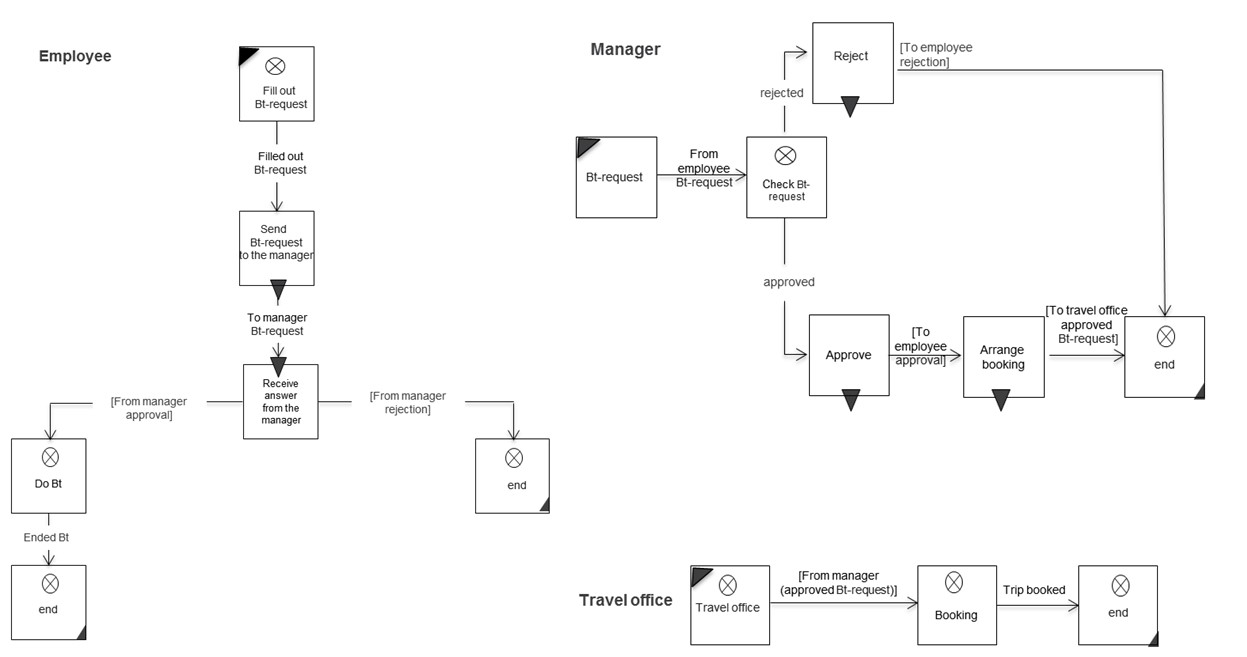
\includegraphics[width=0.7\linewidth]{20181026-Ontologie-Bilder/Grafiken-Ontologie/SUbjectExecution/Vollst-Beispiel}
	\caption[Subject behavior diagram for the subjects ‘employee’, ‘manager’, and ‘travel office’]{Subject behavior diagram for the subjects ‘employee’, ‘manager’, and ‘travel office’}
	\label{fig:vollst-beispiel}
\end{figure}
\end{landscape}
\newpage




\subsection{Extended Behavior}
In order to reduce description efforts some additional specification constructs have been added to PASS. These constructs are informally explained in the following sections. 

\subsubsection{Macros}
Quite often, a certain behavior pattern occurs repeatedly within a subject. This happens in particular, when in various parts of the process identical actions need to be performed. If only the basic constructs are available to this respect, the same subject behavior needs to be described many times.

Instead, this behavior can be defined as a so-called behavior macro. Such a macro can be embedded at different positions of a subject behavior specification as often as required. Thus, variations in behavior can be consolidated, and the overall behavior can be significantly simplified.

The brief example of the business trip application is not an appropriate scenario to illustrate here the benefit of the use of macros. Instead, we use an example for order processing. Figure \ref{fig:macrobehavior} contains a macro for the behavior to process customer orders. After placing the ‘order’, the customer receives an order confirmation; once the ‘delivery’ occurs, the delivery status is updated.

As with the subject, the start and end states of a macro also need to be identified. For the start states, this is done similarly to the subjects by putting black triangles in the top left corner of the respective state box. In our example, ‘order’ and ‘delivery’ are the two correspondingly labeled states. In general, this means that a behavior can initiate a jump to different starting points within a macro.

The end of a macro is depicted by gray bars, which represent the successor states of the parent behavior. These are not known during the course of the macro definition.

\begin{figure*}[ph]
	\centering
	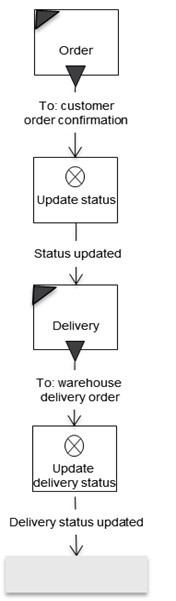
\includegraphics[width=0.2\linewidth]{20181026-Ontologie-Bilder/Grafiken-Ontologie/SUbjectExecution/MacroBehavior}
	\caption[Behavior macro class ‘request for approval’]{Behavior macro class ‘request for approval’}
	\label{fig:macrobehavior}
\end{figure*}

Figure \ref{fig:macrousage} shows a subject behavior in which the modeler uses the macro ‘order processing’ to model both a regular order (with purchase order), as well as a call order.

The icon for a macro is a small table, which can contain multiple columns in the first line for different start states of the macro. The valid start state for a specific case is indicated by the incoming edge of the state transition from the calling behavior. The middle row contains the macro name, while the third row again may contain several columns with possible output transitions, which end in states of the surrounding behavior.

The left branch of the behavioral description refers to regular customer orders. The embedded macro is labeled correspondingly and started with the status ‘order’, namely through linking the edge of the transition ‘order accepted’ with this start state. Accordingly, the macro is closed via the transition ‘delivery status updated’.

The right embedding deals with call orders according to organizational frameworks and frame contracts. The macro starts therefore in the state ‘delivery’. In this case, it also ends with the transition ‘delivery status updated’.

\begin{figure}[ph]
	\centering
	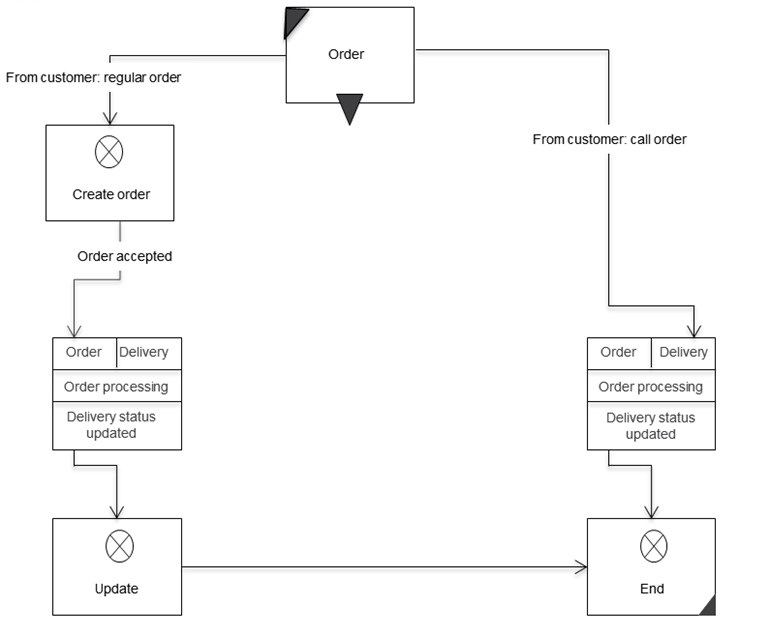
\includegraphics[width=0.6\linewidth]{20181026-Ontologie-Bilder/Grafiken-Ontologie/SUbjectExecution/MacroUsage}
	\caption[Subject behavior for order processing with macro integration]{Subject behavior for order processing with macro integration}
	\label{fig:macrousage}
\end{figure}

Similar subject behavior can be combined into macros. When being specified, the environment is initially hidden, since it is not known at the time of modeling.

\newpage

\subsubsection{Guards: Exception Handling and Extensions} 

\textbf{Exception Handling}\\
Handling of an exception (also termed message guard, message control, message monitoring, message observer) is a behavioral description of a subject that becomes relevant when a specific, exceptional situation occurs while executing a subject behavior specification. It is activated when a corresponding message is received, and the subject is in a state in which it is able to respond to the exception handling. In such a case, the transition to exception handling has the highest priority and will be enforced.

Exception handling is characterized by the fact that it can occur in a process in many behavior states of subjects. The receipt of certain messages, e.g., to abort the process, always results in the same processing pattern. This pattern would have to be modeled for each state in which it is relevant. Exception handlings cause high modeling effort and lead to complex process models, since from each affected state a corresponding transition has to be specified. In order to prevent this situation, we introduce a concept similar to exception handling in programming languages or interrupt handling in operating systems.

To illustrate the compact description of exception handlings, we use again the service management process with the subject ‘service desk’ introduced in section 5.6.5. This subject identifies a need for a business trip in the context of processing a customer order—an employee needs to visit the customer to provide a service locally. The subject ‘service desk’ passes on a service order to an employee. Hence, the employee issues a business trip request. In principle, the service order may be canceled at any stage during processing up to its completion. Consequently, this also applies to the business trip application and its subsequent activities.

Below, it is first shown how the behavior modeling looks without the concept of exception handling. The cancelation message must be passed on to all affected subjects to bring the process to a defined end. Figure \ref{fig:sid-exception} shows the communication structure diagram with the added cancelation messages to the involved subjects.

\begin{figure}[ph!]
	\centering
	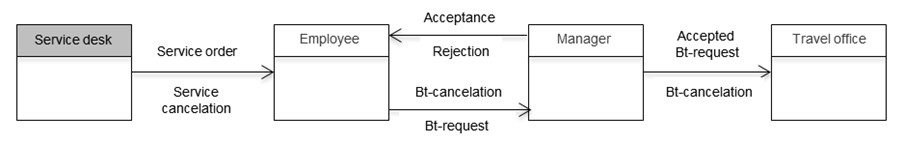
\includegraphics[width=0.7\linewidth]{20181026-Ontologie-Bilder/Grafiken-Ontologie/SUbjectExecution/SID-Exception}
	\caption[Communication structure diagram (CSD) of the business trip application]{Communication structure diagram (CSD) of the business trip application}
	\label{fig:sid-exception}
\end{figure}


A cancelation message can be received by the employee either while filling out the application, or while waiting for the approval or rejection message from the manager. With respect to the behavior of the subject ‘employee’, the state ‘response received from manager’ must also be enriched with the possible input message containing the cancelation and the associated consequences (see Figure \ref{fig:exceptionhandling}). The verification of whether filing the request is followed by a cancelation, is modeled through a receive state with a timeout. In case the timeout is zero, there is no cancelation message in the input pool and the business trip request is sent to the manager. Otherwise, the manager is informed of the cancelation and the process terminates for the subject ‘employee’.


\begin{figure}[ph]
\centering
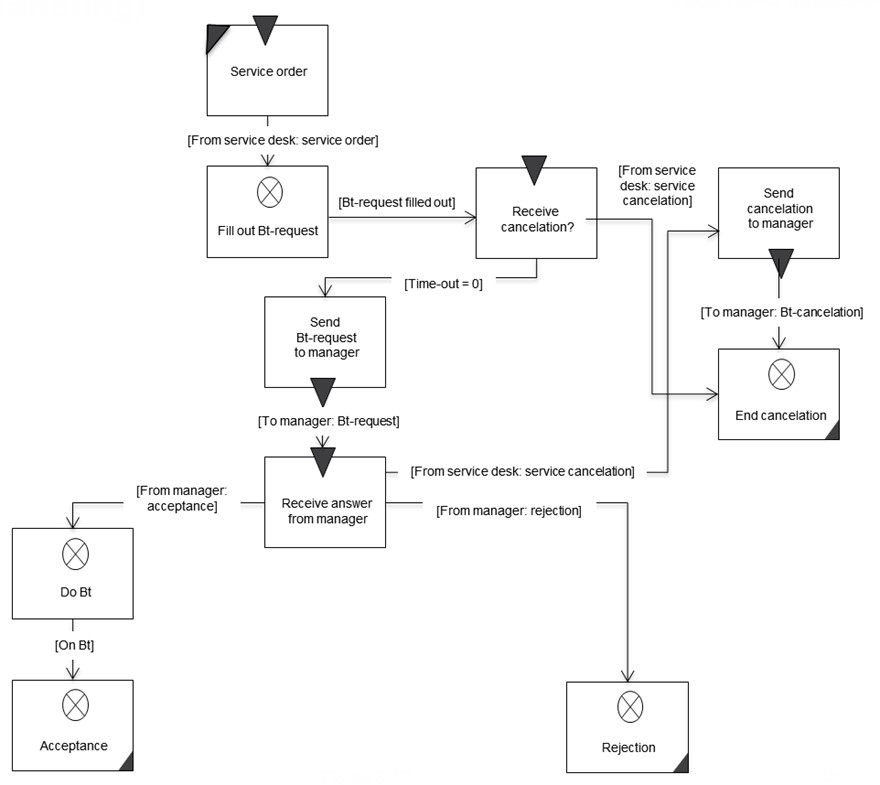
\includegraphics[width=0.7\linewidth]{20181026-Ontologie-Bilder/Grafiken-Ontologie/SUbjectExecution/ExceptionHandling}
\caption[Handling the cancelation message using existing constructs]{Handling the cancelation message using existing constructs}
\label{fig:exceptionhandling}
\end{figure}


A corresponding adjustment of the behavior must be made for each subject which can receive a cancelation message, including the manager, the travel office, and the interface subject ‘travel agent’.

This relatively simple example already shows that taking such exception messages into account can quickly make behavior descriptions confusing to understand. The concept of exception handling, therefore, should enable supplementing exceptions to the default behavior of subjects in a structured and compact form. Figure 5.48 shows how such a concept affects the behavior of the employee.

\newpage

\begin{figure}[ph!]
	\centering
	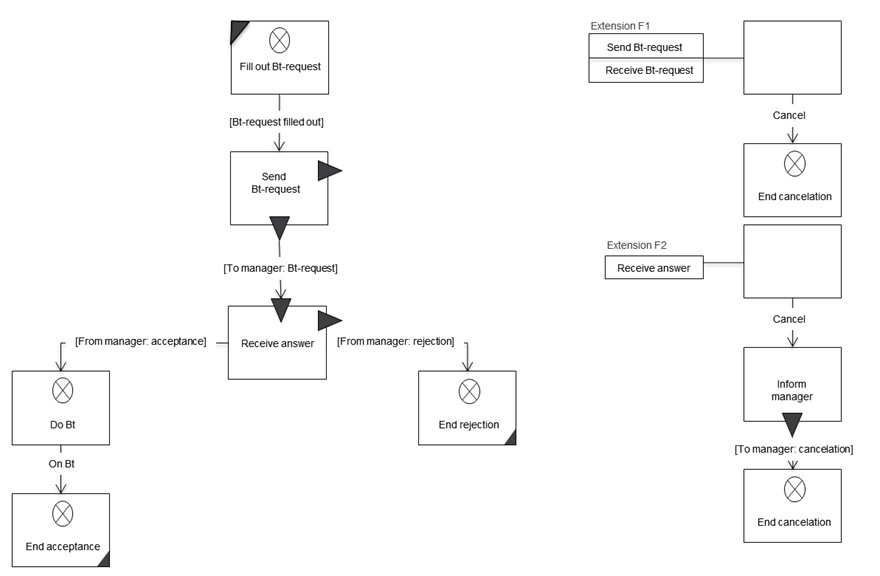
\includegraphics[width=0.7\linewidth]{20181026-Ontologie-Bilder/Grafiken-Ontologie/SUbjectExecution/Extension}
	\caption[Behavior of subject ‘employee’ with exception handling]{Behavior of subject ‘employee’ with exception handling}
	\label{fig:extension}
\end{figure}

Instead of, as shown in Figure \ref{fig:exceptionhandling}, modeling receive states with a timeout zero and corresponding state transitions, the behavioral description is enriched with the exception handling ‘service cancelation’. Its initial state is labeled with the states from which it is branched to, once the message ‘service cancelation’ is received. In the example, these are the states ‘fill out Bt-request’ and ‘receive answer from manager’. Each of them is marked by a triangle on the right edge of the state symbol. The exception behavior leads to an exit of the subject, after the message ‘service cancelation’ has been sent to the subject ‘manager’.

A subject behavior does not necessarily have to be brought to an end by an exception handling; it can also return from there to the specified default behavior. Exception handling behavior in a subject may vary, depending on from which state or what type of message (cancelation, temporary stopping of the process, etc.) it is called. The initial state of exception handling can be a receive state or a function state.

Messages, like ‘service cancelation’, that lead to exception handling always have higher priority than other messages. This is how modelers express that specific messages are read in a preferred way. For instance, when the approval message from the manager is received in the input pool of the employee, and shortly thereafter the cancelation message, the latter is read first. This leads to the corresponding abort consequences.

Since now additional messages can be exchanged between subjects, it may be necessary to adjust the corresponding conditions for the input-pool structure. In particular, the input-pool conditions should allow storing an interrupt message in the input pool.
To meet organizational dynamics, exception handling and extensions are required. They allow taking not only discrepancies, but also new patterns of behavior, into account.\\

\textbf{Behavior Extensions}\\
When exceptions occur, currently running operations are interrupted. This can lead to inconsistencies in the processing of business objects. For example, the completion of the business trip form is interrupted once a cancelation message is received, and the business trip application is only partially completed. Such consequences are considered acceptable, due to the urgency of cancelation messages. In less urgent cases, the modeler would like to extend the behavior of subjects in a similar way, however, without causing inconsistencies. This can be achieved by using a notation analogous to exception handling. Instead of denoting the corresponding diagram with ‘exception’, it is labeled with ‘extension’.

Behavior extensions enrich a subject’s behavior with behavior sequences that can be reached from several states equivocally.

For example, the employee may be able to decide on his own that the business trip is no longer required and withdraw his trip request. Figure \ref{fig:extension} shows that the employee is able to cancel a business trip request in the states ‘send business trip request to manager’ and ‘receive answer from manager’. If the transition ‘withdraw business trip request’ is executed in the state ‘send business trip request to manager’, then the extension ‘F1’ is activated. It leads merely to canceling of the application. Since the manager has not yet received a request, he does not need to be informed.
\newpage
In case the employee decides to withdraw the business trip request in the state ‘receive answer from manager’, then extension ‘F2’ is activated. Here, first the supervisor is informed, and then the business trip is canceled.

\begin{figure}[ph!]
	\centering
	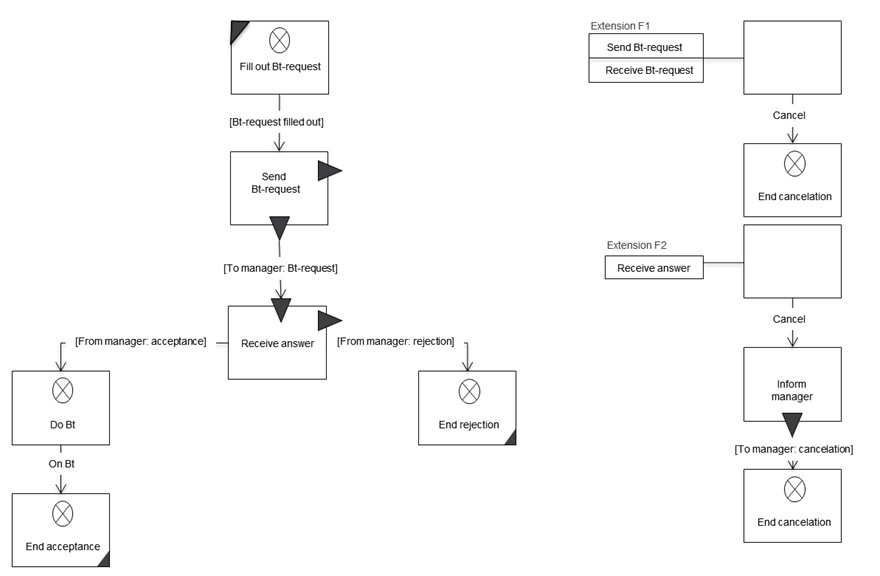
\includegraphics[width=0.7\linewidth]{20181026-Ontologie-Bilder/Grafiken-Ontologie/SUbjectExecution/Extension}
	\caption[Subject behavior of employee with behavior extensions]{Subject behavior of employee with behavior extensions}
	\label{fig:extension}
\end{figure}

\subsubsection{Alternative Actions (Freedom of Choice)} 
So far, the behavior of subjects has been regarded as a distinct sequence of internal functions, send and receive activities. In many cases, however, the sequence of internal execution is not important.

Certain sequences of actions can be executed overlapping. We are talking about freedom of choice when accomplishing tasks. In this case, the modeler does not specify a strict sequence of activities. Rather, a subject (or concrete entity assigned to a subject) will organize to a particular extent its own behavior at runtime.

The freedom of choice with respect to behavior is described as a set of alternative clauses which outline a number of parallel paths. At the beginning and end of each alternative, switches are used: A switch set at the beginning means that this alternative path is mandatory to get started, a switch set at the end means that this alternative path must be completely traversed. This leads to the following constellations:
\begin{itemize}
	\item Beginning is set / end is set: Alternative needs to be processed to the end.
	\item Beginning is set / end is open: Alternative must be started, but does not need to be finished. 
	\item Beginning is open / end is set: Alternative may be processed, but if so must be completed.
	\item Beginning is open / end is open: Alternative may be processed, but does not have to be completed.
\end{itemize}
The execution of an alternative clause is considered complete when all alternative sequences, which were begun and had to be completed, have actually been entirely processed and have reached the end operator of the alternative clause.

Transitions between the alternative paths of an alternative clause are not allowed. An alternate sequence starts in its start point and ends entirely within its end point.

Figure \ref{fig:alternative} shows an example for modeling alternative clauses. After receiving an order from the customer, three alternative behavioral sequences can be started, whereby the leftmost sequence, with the internal function ‘update order’ and sending the message ‘deliver order’ to the subject ‘warehouse’, must be started in any case. This is determined by the ‘X’ in the symbol for the start of the alternative sequences (gray bar is the starting point for alternatives). This sequence must be processed through to the end of the alternative because it is also marked in the end symbol of this alternative with an ‘X’ (gray bar as the end point of the alternative).

\begin{figure}[h!]
	\centering
	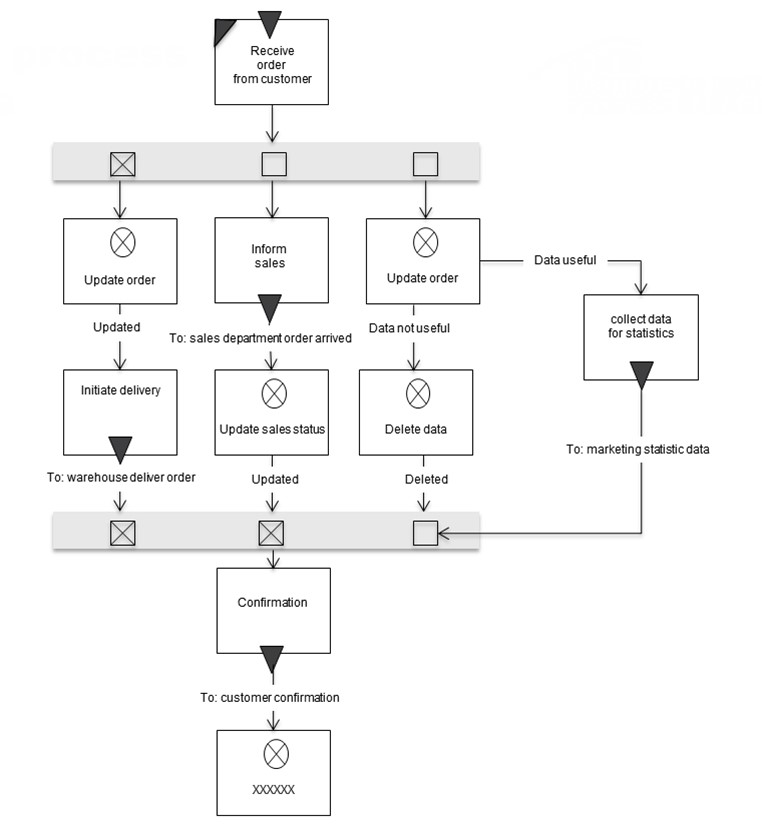
\includegraphics[width=0.7\linewidth]{20181026-Ontologie-Bilder/Grafiken-Ontologie/SUbjectExecution/ALternative}
	\caption[Example of Process Alternatives]{Example of Process Alternatives}
	\label{fig:alternative}
\end{figure}

The other two sequences may, but do not have to be, started. However, in case the middle sequence is started, i.e., the message ‘order arrived’ is sent to the sales department, it must be processed to the end. This is defined by an appropriate marking in the end symbol of the alternatives (‘X’ in the lower gray bar as the endpoint of the alternatives). The rightmost path can be started, but does not need to be completed.

The individual actions in the alternative paths of an alternative clause may be arbitrarily executed in parallel and overlapping, or in other words: A step can be executed in an alternative sequence, and then be followed by an action in any other sequence. This gives the performer of a subject the appropriate freedom of choice while executing his actions.

In the example, the order can thus first be updated, and then the message ‘order arrived’ sent to sales. Now, either the message ‘deliver order’ can be sent to the warehouse or one of the internal functions, ‘update sales status’ or ‘collect data for statistics’, can be executed.

The left alternative must be executed completely, and the middle alternative must also have been completed, if the first action (‘inform sales’ in the example) is executed. It can occur that only the left alternative is processed because the middle one was never started. Alternatively, the sequence in the middle may have already reached its end point, while the left is not yet complete. In this case the process waits until the left one has reached its end point. Only then will the state ‘confirmation’ be reached in the alternative clause. The right branch neither needs to be started, nor to be completed. It is therefore irrelevant for the completion of the alternative construct.
The leeway for freedom of choice with regards to actions and decisions associated with work activities can be represented through modeling the various alternatives—situations can thus be modeled according to actual regularities and preferences.


\newpage

\section{Ontology of Subject Behavior Description}
Each subject has a base behavior (see property 202 in \ref{fig:20190104-simple-elements-and-modellelement}) and may have additional subject behaviors (see class SubjectBehavior in \ref{fig:20190104-simple-elements-and-modellelement}) for macros and guards. All these behaviors are subclasses of the class SubjectBehavior. The details of these behaviors are defined as state transition diagrams (PASS behavior diagrams). These behavior diagrams are represented in the ontology with the class BehaviorDescribingComponent (see figure \ref{fig:20190104-simple-elements-and-modellelement}). The behavior diagrams have the relation belongsTo to the class SubjectBehavior. The other classes are needed for embeddingsubjects into the subject interaction diagram (SID) of a PASS specification (see chapter \ref{OWL-DescriptionSID}).
\begin{figure}[ph]
	\centering
	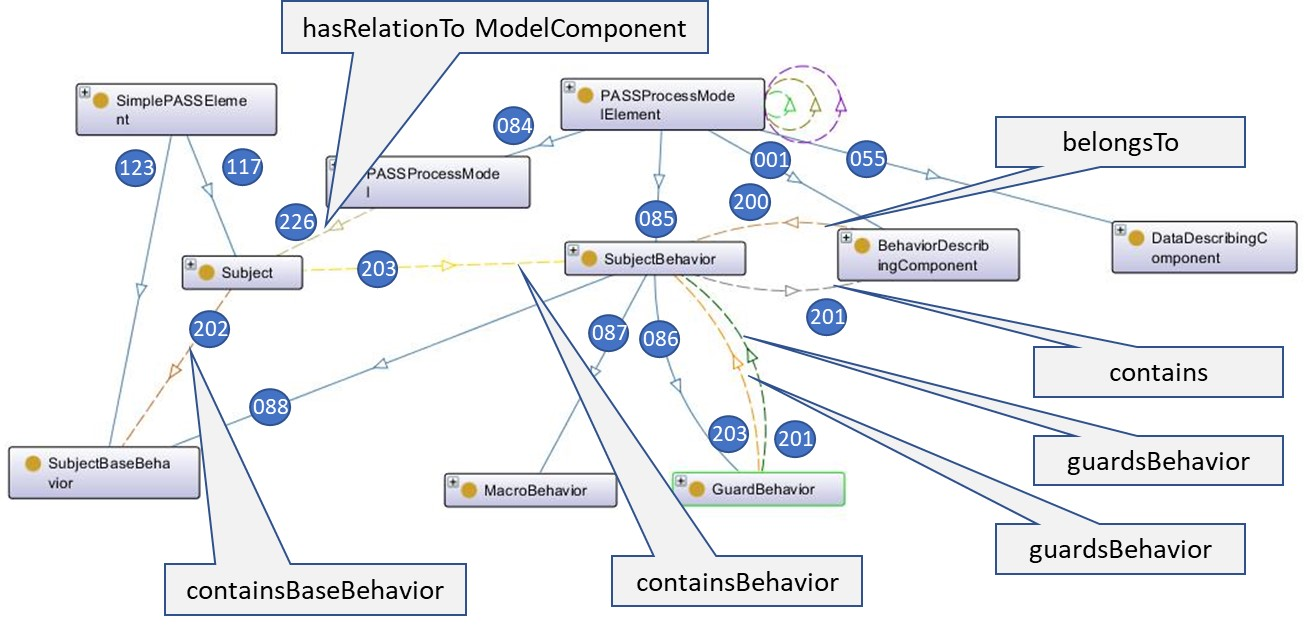
\includegraphics[width=0.9\linewidth]{20181026-Ontologie-Bilder/Grafiken-Ontologie/SUbjectExecution/20190104-SImple-Elements-and-Modellelement}
	\caption[Structure of Subject Behavior Specification]{Structure of Subject Behavior Specification}
	\label{fig:20190104-simple-elements-and-modellelement}
\end{figure}

\newpage

\subsection{Behavior Describing Component}
The following figure shows the details of the claa BehaviorDescribingComponent. This claa has the subclasses Stat, Transition and TranssitionCondition (see figure \ref{fig:20190104-behavior-describing-component}). The subclasses of the state represent the various types of states (class relations 025, 014 und 024 in \ref{fig:20190104-behavior-describing-component}). The standard states are subclasses of the class StandardPASSState (class relations 114, 115 und 116 in \ref{fig:20190104-behavior-describing-component}). The subclass relations 104 and 020 allow that there exist a start state (class InitialStatOfBehavior in \ref{fig:20190104-behavior-describing-component}) and none or several end states (see subclass relation 020 in figure\ref{fig:20190104-behavior-describing-component}) The fact that there must be at least one start state and none or several end states is defined by so called axioms which are not shown in figure \ref{fig:20190104-behavior-describing-component}.
\begin{figure}[ph]
	\centering
	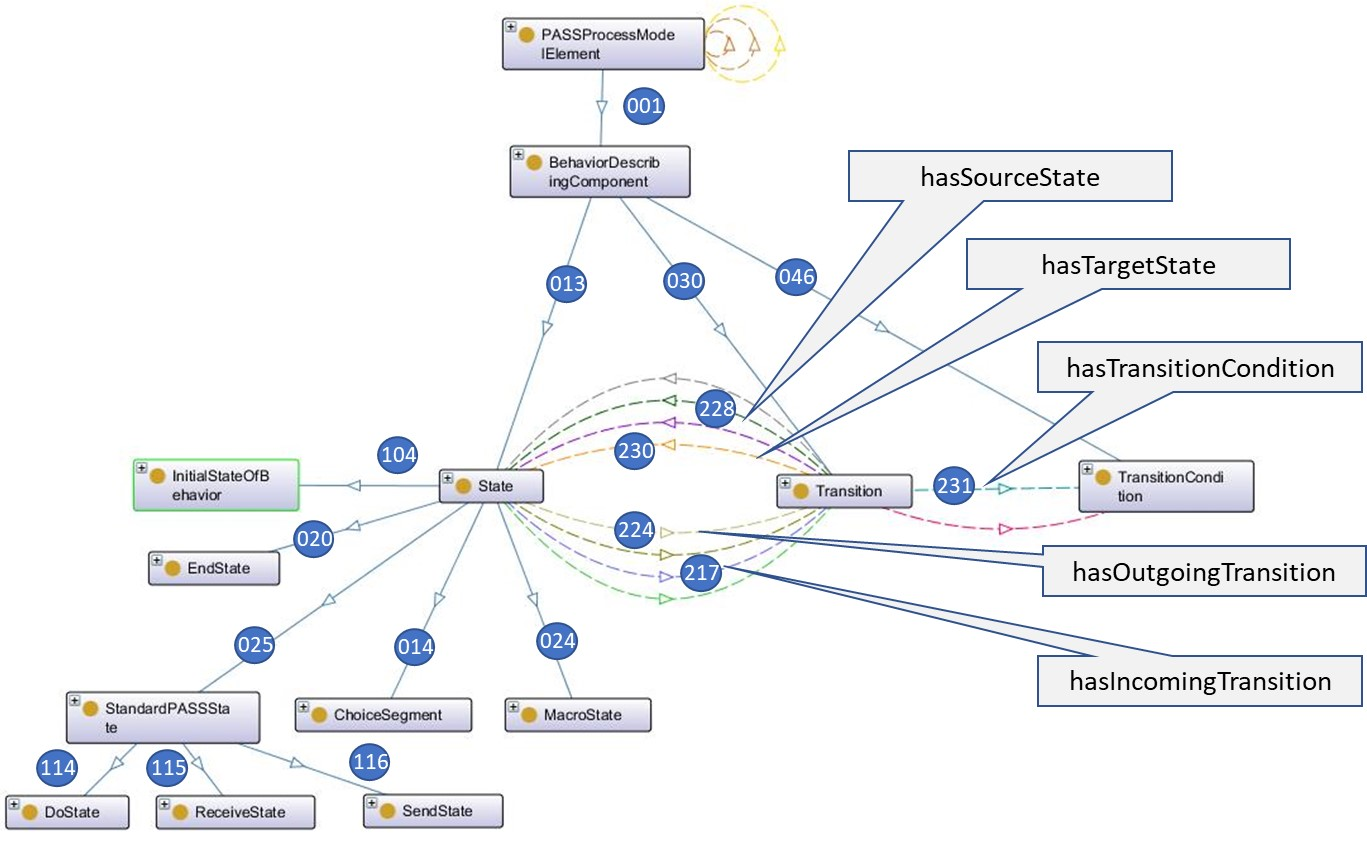
\includegraphics[width=1.0\linewidth]{20181026-Ontologie-Bilder/Grafiken-Ontologie/SUbjectExecution/20190104-Behavior-describing-component}
	\caption[Subject Behavior describingComponent]{Subject Behavior describingComponent}
	\label{fig:20190104-behavior-describing-component}
\end{figure}

\newpage
\subsubsection{Transitions}

\begin{figure}[ph]
	\centering
	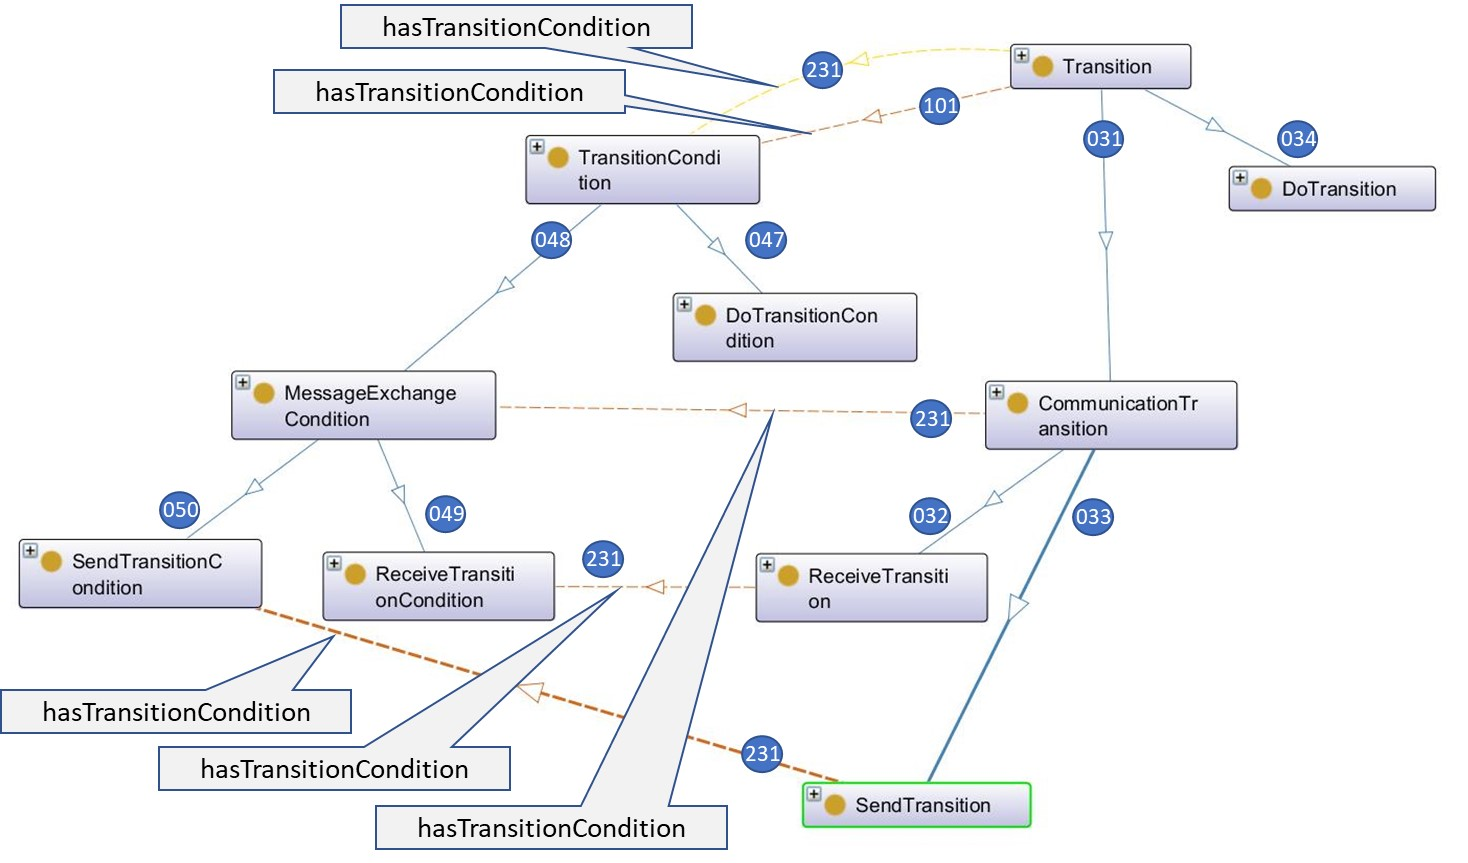
\includegraphics[width=0.7\linewidth]{20181026-Ontologie-Bilder/Grafiken-Ontologie/SUbjectExecution/20190105-Transitions}
	\caption[Details of transitions]{Details of transitions}
	\label{fig:20190105-transitions}
\end{figure}

\newpage

\subsection{Simple Elements for Behavior Description}


\newpage
\subsection{Subject Base Behavior}




\subsection{Macro Behavior}


\subsection{Guard Behavior}



\section{ASM Definition of Subject Execution}